\documentclass[runningheads]{llncs}

\usepackage{graphicx}

\begin{document}

\title{Offline Messenger}

\author{Grigoriu \c Stefan-Cosmin, an 2, grupa E2}

\authorrunning{G. \c Stefan-Cosmin}


\institute{Universitatea "Al. I. Cuza", Informatic\u a Ia\c si, RO
\url{https://profs.info.uaic.ro/~computernetworks/}\\
\email{stefan.grigoriu@info.uaic.ro}}

\maketitle              % typeset the header of the contribution

\begin{abstract}
\^ In aceast\u a documenta\c tie vom introduce subiectul abordat, vom discuta despre motiva\c tia alegerii proiectului propus, implementarea lui, caracteristicile utilizate \^ in cadrul acestuia, conceptele, precum \c si detalii de implementare \c si scenarii de utilizare, iar \^ in final vom concluziona cu ajutorul motiva\c tiei alegerii proiectului, precum \c si cu \^ imbun\u at\u a\c tirile viitoare posibile.
\end{abstract}


\section{Introducere}

Proiectul ales, {\bf Offline Messenger}, cere dezvoltarea unei aplica\c tii ce se bazeaz\u a pe tipul client/server ce permite schimbul de mesaje \^ intre doi, trei sau mai mul\c ti utilizatori conecta\c ti, dar \^ in acela\c si timp s\u a ofere aceea\c si func\c tionalitate \c si c\u atre utilizatorii ce \^ inc\u a nu sunt \^ in momentul trimiterii mesajelor conecta\c ti la server. Astfel, utilizatorilor {\bf offline} le vor fi ar\u atate mesajele primite \^ in momentul conect\u arii la server. O alt\u a func\c tionalitate propus\u a proiectului prezentat este aceea ca utilizatorii s\u a aib\u a posibilitatea de a trimite un r\u aspuns \^ in mod specific la anumite mesaje primite de la al\c ti utilizatori, lucru ce implic\u a necesitatea stoc\u arii unui istoric al mesajelor transmise tuturor utilizatorilor, acest istoric fiind accesibil de c\u atre clien\c ti, la cerere, pentru \c si cu fiecare utilizator \^ in parte.


\subsection{Motiva\c tia}

Apari\c tia internetului a produs schimb\u ari majore \^ in via\c ta oamenilor, fiind un mediu prietenos pentru implementarea aplica\c tiilor de orice fel, de la o simpl\u a comunicare via text sau video, p\^ ana la business-uri online, cloud computing, dezvoltarea inteligen\c tei artificiale, etc. Cu ajutorul internetului reu\c sim s\u a comunic\u am cu persoane aflate la distan\c te foarte mari de noi, \^ in timp real, lucru ce ne u\c sureaz\u a via\c ta de zi cu zi \c si ne men\c tine aproape de cei dragi. Astfel, pentru a putea \^ intelege mai bine \c si a acumula cuno\c stin\c tele necesare program\u arii cu ajutorul protocoalelor de tip TCP/IP, precum \c si pentru a ne dezvolta experien\c ta program\u arii cu ajutorul proceselor-copil/threadurilor \c si socketurilor, am ales crearea unei aplica\c tii de tip {\bf Messenger}, astfel pun\^ and bazele acesteia \c si confrunt\^ andu-ne cu problemele ap\u arute pe parcurs.

\section{Tehnologiile utilizate}

Dat fiind faptul c\u a aceast\u a comunicare prin intermediul aplica\c tiei {\bf Messenger} va trebui realizat\u a cu ajutorul internetului pentru a conecta clien\c tii la un anumit server, am ales folosirea protocolului de tip TCP/IP. Deoarece prin intermediul serverului vor fi conecta\c ti mai mul\c ti utilizatori ce vor efectua opera\c tiuni \^ in paralel, serverul va trebui s\u a fie unul concurent.

\vspace{1cm}

\subsection{Protoclul TCP/IP}

Protocolul TCP/IP a fost ales pentru a fi folosit \^ in acest proiect din mai multe motive, acestea fiind urm\u atoarele:

\begin{itemize}
	\item Deoarece acesta este un protocol orientat pe conexiune, el se ocup\u a de transmiterea \^ in siguran\c t\u a, f\u ar\u a erori, a tuturor octe\c tilor trimi\c si de la ma\c sina surs\u a. 
	\newline
	\item Protocolul se ocup\u a de asemenea \c si de controlul fluxului de informa\c tii pentru ca destinatarul s\u a nu fie inundat cu mesaje mai multe dec\^ at poate procesa, iar astfel octe\c tii sunt transmi\c si \^ in ordinea exact\u a trimiterii, fie c\u a mesajul a fost transmis \^ in unul singur de dimensiune mare, sau mai multe de dimensiuni mici.
	\newline
	\item Dat fiind faptul c\u a \^ in aplica\c tia noastr\u a este necesar\u a o comunicare bidirec\c tional\u a, cu ajutorul nivelului re\c tea ("IP"), pachetele sunt trimise de la o ma\c sin\u a la alta cu ajutorul adresei IP si a unui PORT, comunicarea fiind una full-duplex.
\end{itemize}

\vspace{0.5cm}

\subsection{Baza de date}

Dat\u a fiind necesitatea stoc\u arii informa\c tiilor de tip user, parola, istoric mesaje, etc. pentru fiecare client \^ in parte, o baz\u a de date va trebui folosit\u a. Astfel, la momentul conect\u arii unui client, acesta se poate fie \^ inregistra, fie poate intra \^ in contul s\u au folosind un user \c si o parol\u a \^ inregistrate \^ in tabelul din baza de date. Mai apoi, toate mesajele necitite de acesta \^ ii vor fi ar\u atate, iar noile mesaje ale clientului vor fi memorate \^ in baza de date \^ in istoricul acestuia, precum \c si al destinatarilor.
\newline
Pentru o u\c surin\c t\u a \^ in implementarea unui SGBD, am ales folosirea unui tip de baz\u  a de date embedded, ce nu necesit\u a un anumit server sau o alt\u a configurare, denumit {\bf SQLite}, fiind una dintre cele mai folosite din lume \c si av\^ and libr\u arii native C.

\vspace{1cm}

\section{Arhitectura aplica\c tiei}

\begin{figure}
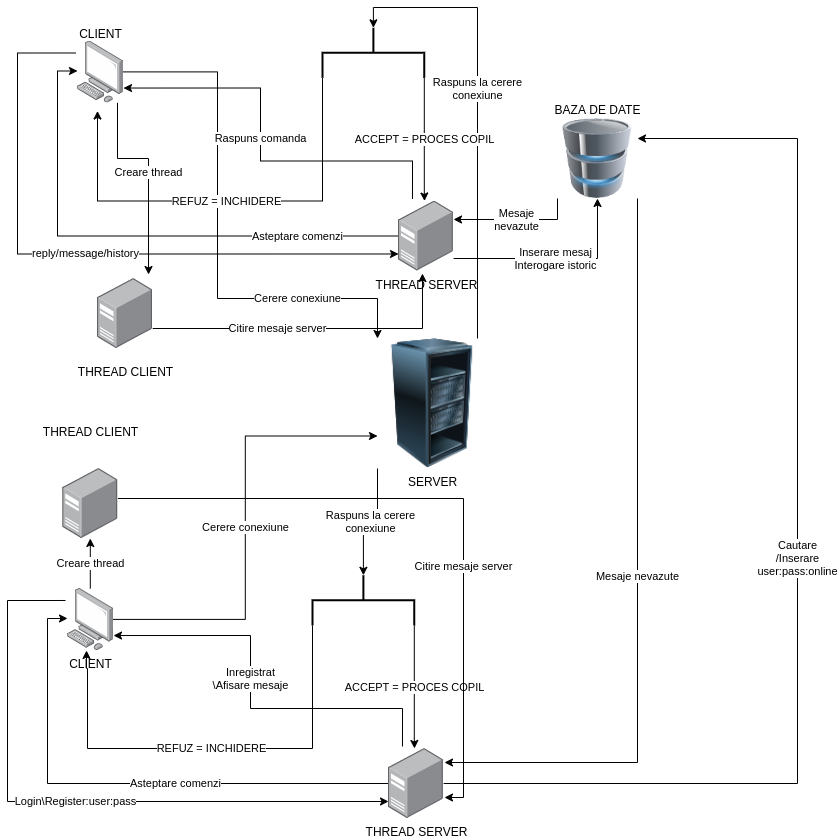
\includegraphics[width=\textwidth]{project.png}
\caption{Diagrama cu arhitectura aplica\c tiei} \label{fig1}
\end{figure}


\begin{figure}
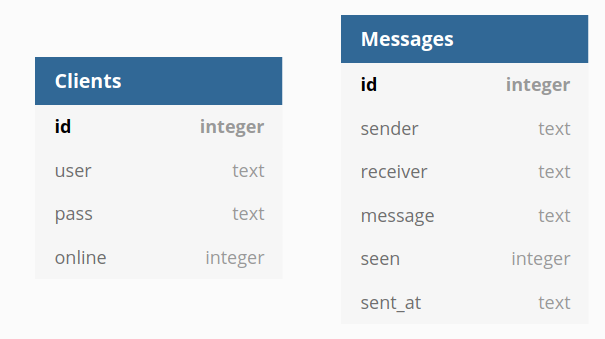
\includegraphics[width=\textwidth]{database.png}
\caption{Tabele baza de date} \label{fig1}
\end{figure}

Aplica\c tia prezentat\u a \^ in diagrama de mai sus ilustreaz\u a comunicarea \^ intre doi clien\c ti, comunicare posibil\u a prin intermediul serverului \c si a proceselor-copil create de acesta. \^ In practic\u a, \^ in momentul cererii de conectare utiliz\^ and protocolul TCP/IP si socketurile, serverul, \^ in caz de acceptare a conexiunii, se folose\c ste de procese-copil sau threaduri  pentru a \^ indeplini cererile fiec\u arui client, iar tot prin acest proces-copil/thread faciliteaz\u a comunicarea clien\c tilor \c si stocarea mesajelor cu ajutorul unei baze de date.

\section{Detalii de implementare}

Pa\c sii pentru a utiliza aplica\c tia propus\u a, {\bf Offline Messenger}, sunt urm\u atorii:

\begin{enumerate}
	\item Serverul este pornit \c si a\c steapt\u a conexiuni la IP-ul propriu \c si PORT-ul desemnat;
	\newline
	\item Clientul este pornit, iar adresa \c si PORT-ul sunt specificate;
	\newline
	\item Clientul trimite o cerere de conectare c\u atre server, cerere ce va fi acceptat\u a, iar serverul va crea un thread pentru comunicarea cu clientul;
	\newline
	\item Clientul poate folosi doar comanda 'login:user:pass' sau 'register:user:pass';
	\begin{enumerate}
		\item Dac\u a clientul a ales comanda {\bf register}, c\^ ampurile user \c si pass vor fi introduse \^ in baza de date, cu condi\c tia ca userul s\u a nu fie deja existent, iar mai apoi userul va fi online;
		\item Dac\u a clientul a ales comanda {\bf login}, c\^ ampurile user si pass vor fi verificate cu toate conturile existente \^ in baza de date, iar \^ in caz de potrivire, userul va fi online, iar daca nu, atunci va putea \^ incerca din nou;
		\newline
	\end{enumerate}
	\item Dupa ce a fost logat, clientul va crea un thread ce se va ocupa de citirea mesajelor de la server \c si i se vor afi\c sa pe ecran toate mesajele primite c\^ at timp a fost offline. Acesta poate scrie \^ in fereastr\u a pentru a vedea comenzile disponibile sau poate folosi direct comenzile {\bf 'history:all'} sau {\bf 'history:user'}, {\bf 'reply:[data timp]'}, {\bf 'msg:user'} sau {\bf 'quit'};
	\begin{enumerate}
		\item La comanda {\bf 'history:all/user'}, clientul va alege fie s\u a vad\u a tot istoricul conversa\c tiilor lui cu to\c ti utilizatorii cu care a comunicat, fie poate alege s\u a vad\u a doar istoricul mesajelor cu un anumit utilizator;
		\item La comanda {\bf 'reply:[data timp]'}, clientul va r\u aspunde la mesajul selectat cu ajutorul datelor trimiterii acestuia, ce apar pe ecran, iar r\u aspunsul va fi stocat \^ in baza de date \c si trimis persoanei ce a scris mesajul;
		\item La comanda {\bf 'msg:user'}, clientul va trimite un mesaj privat userului specificat, iar cel din urm\u a va fi notificat, mesajul ap\u ar\^ andu-i pe ecran \^ impreun\u a cu persoana data, ora \c si numele utilizatorului ce a trimis mesajul;
		\item La comanda {\bf 'quit'} clientul este delogat, threadurile din client se vor \^ inchide \c si userul va fi trecut offline \^ in baza de date, iar mesajele noi vor fi salvate \c si afi\c sate la urm\u atorul login;
		\newline
	\end{enumerate}
\end{enumerate}

	La final, dup\u a \^ inchiderea clientului, threadurile se vor opri \c si nu vor exista procese zombie. \^ In caz c\u a serverul va avea probleme(pan\u a de curent, etc.), opera\c tiunile neterminate nu vor fi trecute \^ in tabelurile din baza de date.

\section{Concluzii}

	\^ In concluzie, proiectul propus, {\bf Offline Messenger}, este unul ce necesit\u a bazele program\u arii deprinse din re\c telele de calculatoare, mai exact de ajutorul proceselor-copil, comunic\u arii cu ajutorul socketurilor, protocoalelor de comunicare, threadurilor, dar care \^ in acela\c si timp vine cu nout\u a\c ti precum implementarea unei baze de date pentru stocarea mesajelor \c si utilizatorilor, \^ in acela\c si timp \^ inv\u a\c t\^ andu-ne bune practici de programare.

\subsection{\^ Imbun\u at\u a\c tiri}

	\^ In cazul unei aplica\c tii de tip {\bf Messenger}, foarte multe \^ imbun\u at\u a\c tiri \^ ii pot fi aduse, \^ incep\^ and de la posibilitatea trimiterii diferitelor fi\c siere \^ intre utilizatori precum documente sau fotografii, implementarea unui {\it voice-chat} \c si a unei interfe\c te grafice sau folosirea unei camere web, pana la criptarea tuturor conversa\c tiilor pentru o siguran\c t\u a \c si intimitate  sporit\u a a utilizatorilor.
	
	\vspace{0.5cm}
	
Codul proiectului se g\u ase\c ste pe GitHub, la link-ul nr 3. din Bibiliografie.

\begin{thebibliography}{8}
\bibitem{ref_url1}
TCP/IP, \url{https://ro.wikipedia.org/wiki/TCP/IP}

\bibitem{ref_url2}
Computer Networks, \url{https://profs.info.uaic.ro/~computernetworks/}

\bibitem{ref_url3}
Github Repository, \url{https://github.com/grigoriucosmin/CN{\_}Project/}

\end{thebibliography}
\end{document}
